\chapter{Robotics applications}



\section{Introduction}

The actions a robotic arm can take decide its usefulness. To assist a person in their everyday lives, the arm should be able to, among other things, manipulate objects or interact with machines. To assist in an industrial context, it must be able to use the tools necessary for the task and to be reliable.

What we call applications within ALFRED are the pieces of software that implement the possible actions of the robotic arm. As we presented in a prior chapter, they live in the Userspace where any user is free to implement their applications for their use cases.

We present two applications that were developed to add capabilities to the robotics platform: writing and drawing, and object grasping and manipulation.



% \section{Related work}

% TODO (main related works section)

% \cite{mit_rfusion}
% \marginfig{mit_rfid}

% \cite{quayola_sculpture}
% \marginfig{robot_sculpture}



\section{Writing and drawing}


\subsection{Introduction}

Writing is a complex motor task that children take years to do properly. Drawing is even more complicated, and becoming an artist capable of expressing their thoughts in paper or a digital format is a lifelong endeavor.

A robot can learn these skills by learning the movements once without needing time to practice. Writing and drawing can be useful in automation, where a factory would want to create custom handwritten notes, or sign papers with a pen automatically. It can also help people who can't write by themselves, and don't want to, or can't, transition completely to digital media.


% \subsection{Related work}

% % XXX: related_work


\subsection{Contribution}

\subsubsection{Concept}

This application uses the robotic arm to write text autonomously. It transforms its input text into a sequence of movements of the robotic arm, thus enabling the robot to write on any flat surface, independent of orientation.

The original gripper could not grasp the pen efficiently enough to do continuous writing, so we developed a custom mount for the pen, taking advantage of the provided schematics for the arm's end effector.

% TODO: schematic of the pen mount

The system was then adapted to use the robotic arm to draw line art of images \ref{fig:writing_and_drawing}.

\begin{figure}[h]
    \centering
    \includegraphics[height=7cm]{images/writing.png}
    \hspace{1cm}
    \includegraphics[height=7cm]{images/drawing.png}
    \caption{Writing and drawing}
    \label{fig:writing_and_drawing}
\end{figure}

\subsubsection{Implementation}

\paragraph{Writing}

The API for the writing application takes in a string of the letters to write. It uses a mapping between letters and an array of robot instructions. These robot instructions are numbers and booleans, whose structure is adapted from the API of the robotic arm to be more comprehensible to the programmer. This structure is as follows:

\begin{itemize}
    \item 6 numbers for x, y, z, roll, pitch, yaw. These values are not interpreted as absolute movements relative to a fixed point in space but as relative to the actual position of the arm.
    \item 1 number for the radius of the movement. If the radius is 0, the movement will be a straight line. If it is bigger than 0, the movement will be a curve with the specified radius.
    \item 1 boolean to specify if the radius is in degrees or radians.
\end{itemize}

% TODO: add figure of coord space

Here is an example for the letter D:

\begin{lstlisting}[language=Python, caption=Example for the letter D]
mapping = {
# ...
    "D": [
            # Starting pen up, go to the top left corner
            [10, 0, 0, 0, 0, 0, 0, False],
            # Lower the pen to the paper
            [0, 0, 5, 0, 0, 0, 0, False],
            # Draw the left bar of the D
            [-10, 0, 0, 0, 0, 0, 0, False],
            # Raise the pen
            [0, 0, -5, 0, 0, 0, 0, False],
            # Go back to the top left corner
            [10, 0, 0, 0, 0, 0, 0, False],
            # Lower the pen again
            [0, 0, 5, 0, 0, 0, 0, False],
            # Draw the semi-circle of the D
            [0, 7, 0, 0, 0, 0, 7, False],
            [-10, 0, 0, 0, 0, 0, 7, False],
            [0, -7, 0, 0, 0, 0, 0, False],
            # Raise the pen and prepare for the next letter
            [0, 10, -5, 0, 0, 0, 0, False],
        ],
# ...
}
\end{lstlisting}

The instructions in the mapping use a relative notation, but the performance of moving with only relative motions was not sufficient for the needs of the application. It added delays from calculating the absolute position internally and the movement was choppy. To correct this issue, we store the arm's position at the beginning of each sentence and calculate the absolute position from the relative movements for each robot instruction.

\paragraph{Drawing}

Using the same system as writing as a base, we added the possibility for the arm to draw line art of images. This feature uses images in the Scalable Vector Graphics (SVG) format to extract and draw line art. Images in the SVG format are not described as a matrix of pixels, but rather a series of lines described by mathematical equations. This normally allows the images to be scaled up or down infinitely, but in our case, we use these equations as guides for the trajectory the robot should use to draw the picture.

We support a subset of the SVG format. The supported path instructions are:

\begin{itemize}
    \item MoveTo, or M: move the cursor to the specified position without writing
    \item LineTo, or L: move in a straight line
    \item CurveTo, or C: move in an arc as described by a Bezier curve
    \item ClosePath, or Z: go back to the place the cursor started writing
\end{itemize}

SVG files are pre-processed by hand to remove all unnecessary information. Only the path attributes are kept, and they are formatted to have one command per line. In code, the pre-processed file is parsed into an array containing each command in order. The commands are then translated into the same type of robot instructions as writing. For circles and lines, we first translate the command into a mathematical equation which we then sample according to a manually defined, arbitrary precision level.

This translation essentially creates the same value as the alphabet mapping, where here the key is the id of the drawing and the value is a much more complex array of robot instructions.

% \subsubsection{Evaluation}

\subsection{Conclusion}

\subsubsection{Applications and use cases}

Enabling a robotic arm to write allows anyone with such equipment to write or draw autonomously. This feature allows users to write text on paper without their hands, which can be useful for impaired users or in multitasking situations. This application can also be used to automate writing in a factory or small business. With drawing, company logos or signatures can also be automated.

\subsubsection{Limitations}

One of the drawbacks of our approach is speed. Due to the precise nature of writing, movements need to be slow or the letters produced by the arm are not well drawn, curved or slanted.

Another limitation is the complexity of the setup required. This is caused by the absence of any feedback mechanism on the pen and pen mount. The drawing surface needs to be on a perfectly flat and level surface because the pen cannot adapt itself to the surface. As an extension of this problem, careful calibration is required to make writing work. The pen needs to be placed precisely on the axis perpendicular to the drawing surface (Z-axis calibration). Too high and it will not make contact when writing, too low and it will be forced into the writing support and break. The plane of the robot end effector needs to be perfectly parallel to the plane of the writing surface, or it could progressively go away or towards the surface when writing (XY-axis calibration). This problem can be mitigated by using a large pen like a whiteboard marker and a soft writing surface, so that the pen can dig into the surface a little bit and still write, but it is not an elegant nor viable solution.

\subsubsection{Future works}

One of the possible improvements that can be done to this application is the automation of drawing. Currently, only SVG images are supported, and they have to be pre-processed manually. With edge finding and line fitting algorithms, we could transform any image into lines and then into mathematical equations that could be sampled to give robot instructions.

Another improvement would be the integration of hand writing. By mixing together drawing and writing, we could be able to interpret a user's hand writing as a drawing and use it in our alphabet mapping to replace the original simple letters by custom hand writing. This would improve the system for writing automation since the writing would be much more visually appealing. The system could then be used to automate the writing of custom sentences e.g. for notes.

Finally, to correct the limitation of the writing surface, we could integrate a bed levelling application (which was already developed on ALFRED) to find the location and orientation of the writing surface, removing the need for Z- and XY-axis calibration.



\section{Object grasping and manipulation}


\subsection{Introduction}

Robotic arms traditionally use hardware attached to their end effectors to interact with their environments. When a robotic arm is used to automate welding, for example, it will be equipped with a tool specifically made for this application.

However, in flexible environments such as homes or research laboratories, tasks are more varied than in assembly chains. Using the same approach as in factories would require tools to be changed too often, or specific tools to be made for every variation of a task or environment. Instead, by giving the robotic arm the capability to grasp and manipulate objects, we can make it adapt to many more environments and tasks.


% \subsection{Related work}

% % XXX: related work


\subsection{Contribution}

\subsubsection{Concept}

This application consists of looking for a specific object in a radius around the robotic arm and grasping it once it is found. The operator can then manipulate the object with the robotic arm through voice commands.

First, an object type has to be registered. This can be done at the application's start or during its execution. The robotic arm will then enter \lstinline{scanning mode}: in a loop, it will look at its surroundings section be section to look for the object.

When the object is detected, the application enters \lstinline{homing mode}. In homing mode, the arm centers the camera on the detected object. It starts off with big movements to get close as fast as possible, then uses smaller and smaller movements the closer it gets.

Once homed on the object, the robotic arm begins its approach for grasping. Using camera color frames, it checks that it is still centered on the object. Using camera depth frames, it detects how close it is to the object. Once it is close enough, it closes the gripper. Grasping force is estimated from the depth frames by finding the approximate size of the object. To verify the object has been grasped correctly, we look at the value of the current going to the gripper: a higher value than normal means the gripper is applying force to the object, and therefore that is has grasped it.

If the robotic arm grasped the object successfully, it can then await further commands via the voice interface. Possible commands are to move the object in a certain direction, to hand it to the operator, or to place it back on the experiment space \ref{fig:grasping_cup}.

If at any point in time the system loses the object, the arm executes its \lstinline{return sequence}, getting back into position for scanning.

\begin{figure}[h]
    \centering
    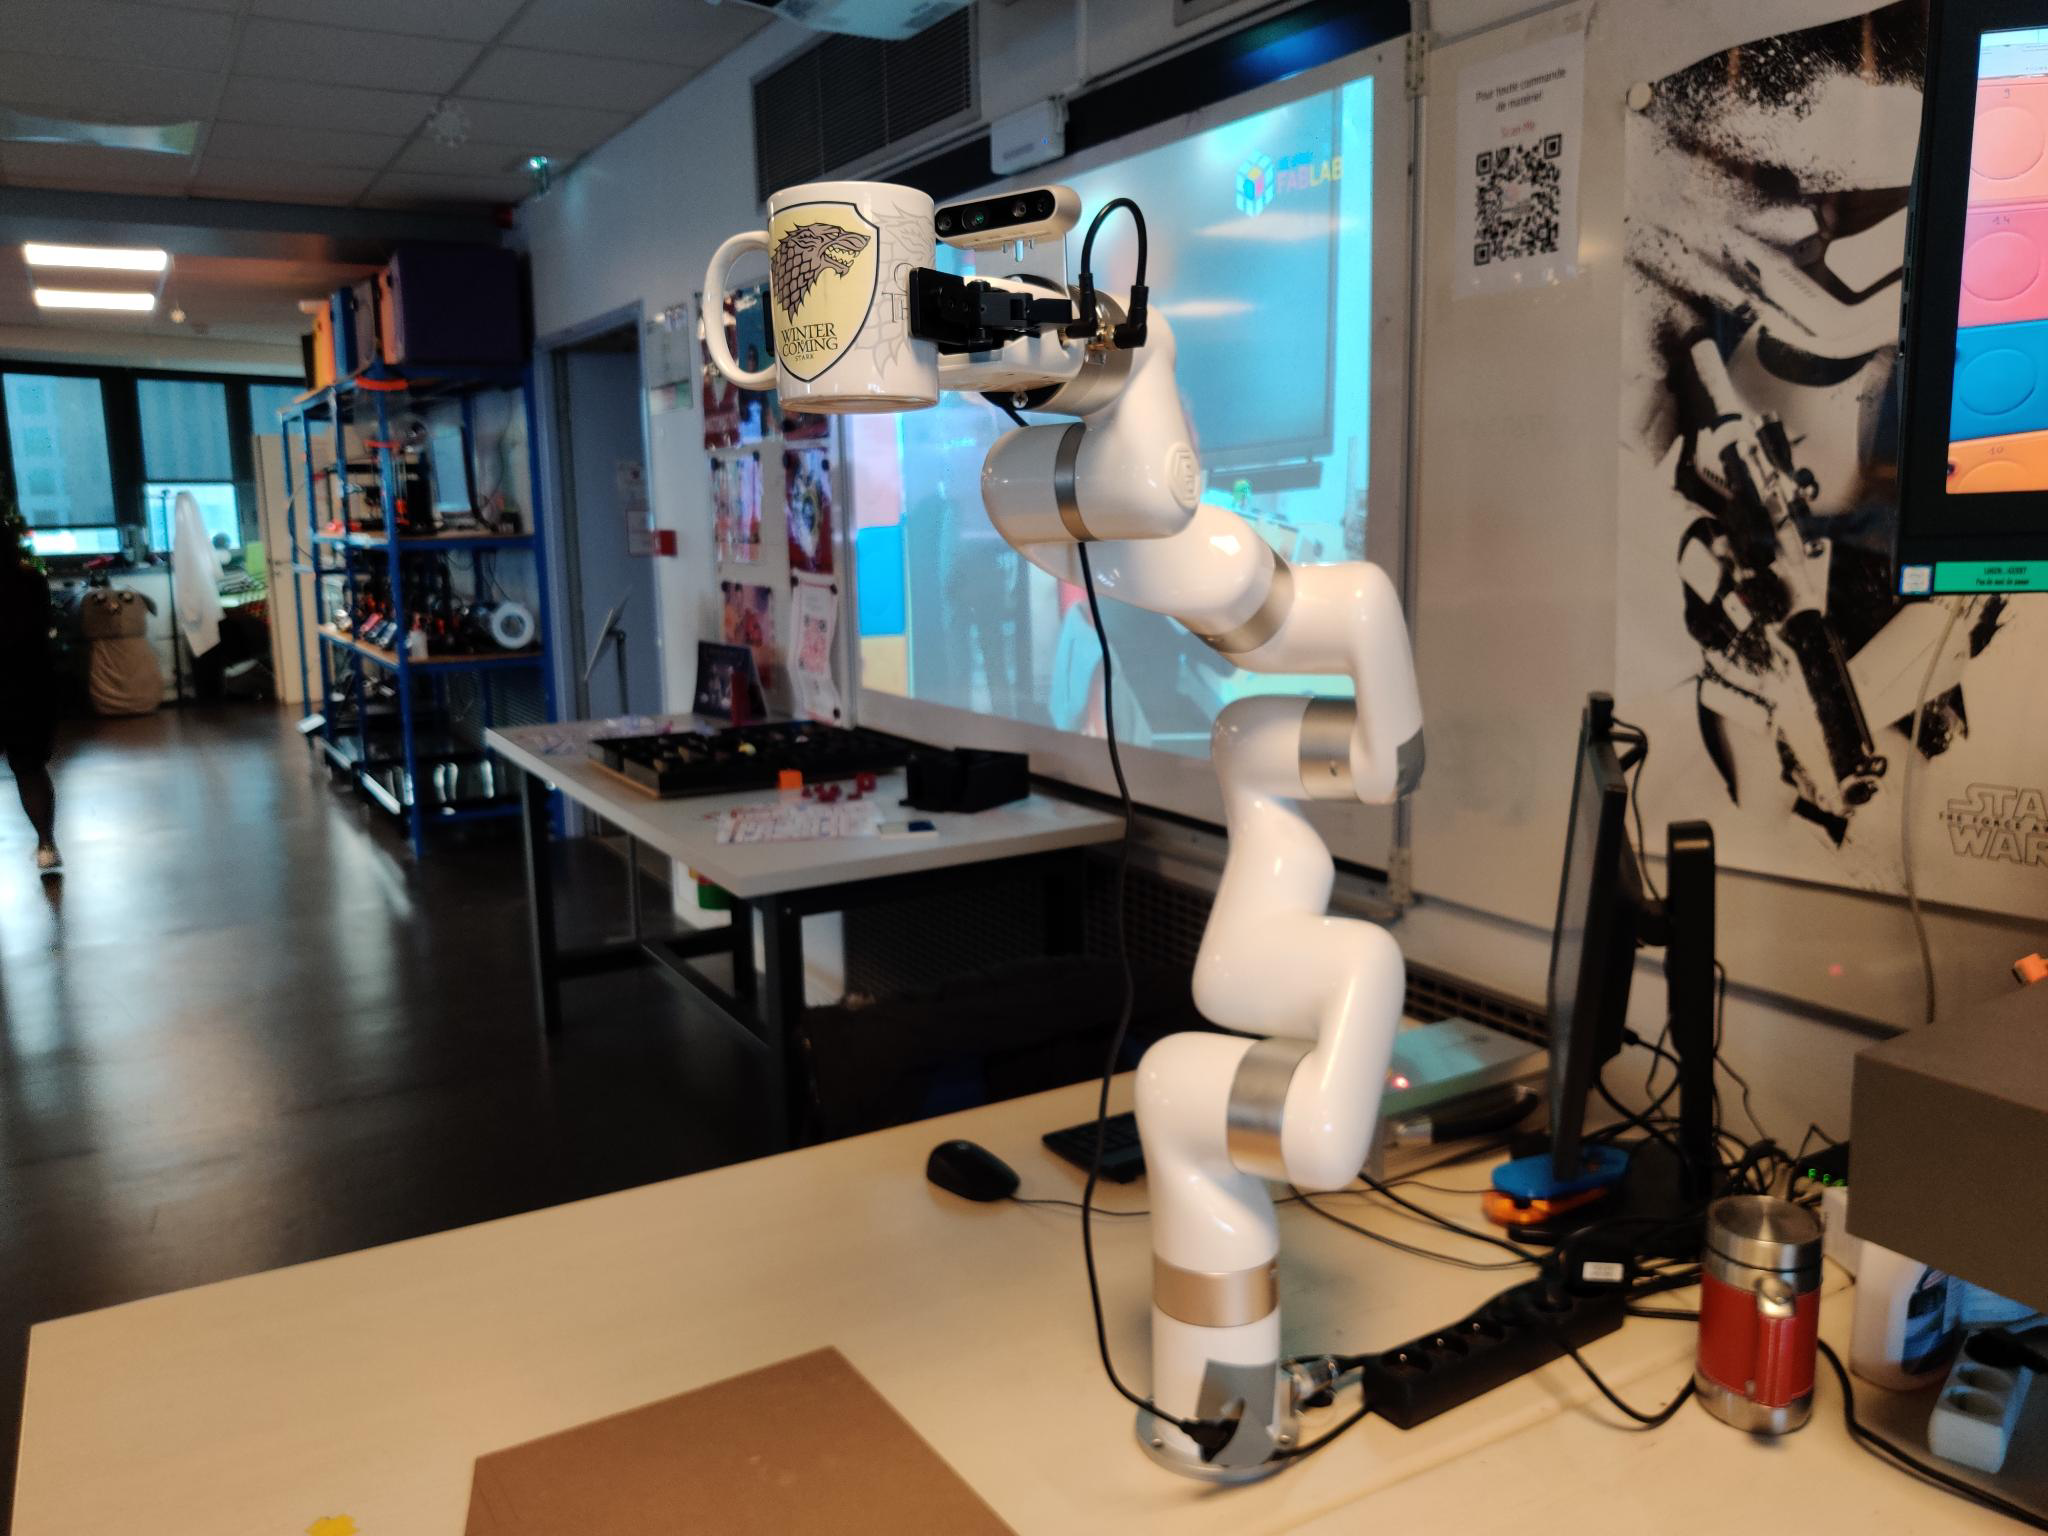
\includegraphics{images/grasping_cup.png}
    \caption{Robot arm grasping a cup, ready to accept commands for manipulation}
    \label{fig:grasping_cup}
\end{figure}

\subsubsection{Implementation}

\paragraph{Starting and interacting with the application}

At its base level, the application is called via an API route within ALFRED. The object to grasp can be given when starting the application or left blank, in which case the arm will not scan for any object. The target object can be changed during execution with another API route. Within ALFRED, applications are run as processes and therefore cannot normally be interacted with\sidenote{Contrary to threads, processes' memories are kept separate which renders memory sharing impossible and thus makes communication harder.}. We thus implemented two-way communication within the application using Python's multiprocessing Pipes. This allows runtime modification of grasping targets.

\paragraph{Image detection}

We use a deep learning image detection algorithm to detect the objects on the experiment surface. We chose to use YOLOv5\cite{yolov5} because of its performance and the fact that only boxing was necessary for this application. YOLOv5 also enables the applications to run on hardware without GPU acceleration with smaller models that can run on the CPU, which increases compatibility and convenience for development. Color frames from the camera are processed by the YOLOv5 model in a separate thread and are used in the decision loop of the application to search for and grasp objects.

\paragraph{Scanning mode}

Modes are determined by flags which are set or unset depending on the current mode, and change the behavior of the application in the decision loop. When the application is started, it automatically enters scanning mode. In scanning mode, the arm circles through a set of positions to search the experiment space for the target object. These positions are determined by linearly sampling values between two points. These points are the extremes of where the arm can move without colliding with its environment, specifically for its first joint. The result is that the arm moves in a semi-circle within the experiment space, and stops at each position for one second to scan for an object, in an infinite loop.

\paragraph{Homing mode}

When the target object has been found, homing mode is activated. Because the object can be anywhere within the camera frame when it is detected, it is necessary to place it in a known position within the frame to continue with the grasping operation. We call this operation homing. In homing mode, the system will try to center the target object within the camera frame. To do so, we calculate the difference in positions between the target object and the center of the frame, expressed with an \lstinline{x} value for height and \lstinline{y} value for width. We then calculate the necessary movement of the arm with a linear scaling. The movement of the arm is not always perfect, so we continue to home into the object until it is centered.

\paragraph{Grasping}

Currently, grasping mode and the behavior of the robot after grasping are not implemented.

% ??? -> put in future works

\paragraph{Return sequence}

If the object is lost during homing or grasping mode, meaning the object moved, or there was a detection error after the object was first detected, the robot needs to reset its position to begin scanning again. To do so, we execute a return sequence which places the robot back into its scanning position, and we also set the current mode back to scanning. The current rotation along the points defined for scanning mode is kept the same, so the robot can continue where it left off in its scanning after being interrupted by the detection of the target object.

% TODO: flow graph of grasping app


% \subsubsection{Evaluation}


\subsection{Conclusion}

\subsubsection{Applications and use cases}

A robot with grasping capabilities can be used at home, at work in research laboratories and FabLabs. With its ability to manipulate objects and tools, the robotic arm could help with tasks such as soldering, or screwing. It could automate repetitive manual tasks, such as product assembly, and assist in cleaning or sorting. It can either be controlled directly or be made to memorize the movements for a task after being directed once.

\subsubsection{Limitations}

Currently, object grasping is not yet implemented in the application. Work has been done to prepare this implementation however, and we found that grasping methods often require complex deep learning models to be reliable. We humans learn the mechanics of grasping by experience, but robots need to learn representations of objects to find where to grab. To obtain these representations, we need a large amount of data and powerful computers for training. The training and deployment complexity make it impractical to adapt to new use cases and situations.

The equipment can also limit the efficiency of the application: the gripper being a classic "pincer" gripper reduces the stability when grasping certain items in round shapes for example.

\subsubsection{Future works}

For the future, we plan to fully implement grasping and after-grasping behavior. This involves creating a basic algorithm for grasping with limited capabilities at first, and then using deep learning to teach the robotic arm to grasp more complex items. Once grasping is implemented, we can create a recording mechanism to memorize tasks to automate.

To solve the problem of the gripper, we could replace our pincer gripper with a soft robotics gripper using pneumatics. This type of gripper mimics the human hand more closely and is more adapted to more organic shapes.



\section{Conclusion}

ALFRED uses applications to implement functionality for the robotic arm. We developed two applications to demonstrate the possibilities of our robotics middleware.

We created writing to familiarize ourselves with the API of the system, and later expanded on the application to implement drawing and enable the user to replicate handwriting, signatures, and SVG images.

We started to develop object grasping and manipulation to turn the robotic arm into a polyvalent assistant capable of interacting with its environment and aid in automating manual tasks.

We found that applications fulfilled our criteria for ease of integration and development through this experimentation.
